% prime_en.tex — Edges of Counting and Computation — Prime
% Compiler: XeLaTeX or pdfLaTeX
\documentclass[12pt,a4paper]{article}
\usepackage{amsmath,amssymb}
\usepackage{graphicx}
\usepackage{booktabs}
\usepackage{array}
\usepackage[margin=2.2cm]{geometry}
\usepackage{xcolor}
\usepackage{float}
\usepackage{hyperref}
\usepackage{fancyhdr}

\pagestyle{fancy}
\fancyhf{}
\fancyhead[L]{\small Edges of Counting and Computation — Prime}
\fancyhead[R]{\small M. N. Al-Jabri (2026)}
\fancyfoot[L]{\scriptsize Abdulla M. N. Al-Jabri | ORCID: 0009-0003-3319-3822}
\fancyfoot[C]{\scriptsize Zenodo DOI: to be assigned}
\fancyfoot[R]{\small \thepage}
\renewcommand{\headrulewidth}{0.4pt}
\renewcommand{\footrulewidth}{0.4pt}

\fancypagestyle{firstpage}{
  \fancyhf{}
  \fancyfoot[C]{\small Abdulla M. N. Al-Jabri — Edges of Counting and Computation — Prime — \thepage}
  \renewcommand{\headrulewidth}{0pt}
  \renewcommand{\footrulewidth}{0pt}
}

\title{\textbf{Edges of Counting and Computation — Prime}\\
\large Cross-Stage Empirical Synthesis ($A \rightarrow D$) up to $10^9$}
\author{Abdulla Mohammed Nasser Al-Jabri \\
Sana'a, Republic of Yemen \\
ORCID: 0009-0003-3319-3822 \\
Email: \texttt{jabri62018@gmail.com} \\
Portal: \url{https://jabri-com.vercel.app} \\
Zenodo DOI: to be assigned on deposit}
\date{November 21, 2026}

\begin{document}
\maketitle
\thispagestyle{firstpage}

\begin{center}
\textbf{We count primes, compute their edges (gaps), and test whether they carry structure or memory.}
\end{center}

% ==========================================
\begin{abstract}
This paper presents a cross-stage computational synthesis ($A \rightarrow D$) investigating the statistical and structural behavior of consecutive prime gaps $g_n = p_{n+1} - p_n$ up to $N = 10^9$. Using a strictly frozen protocol across four ascending stages ($10^6, 10^7, 10^8$, and $10^9$), we track the prime counting function $\pi(x)$, logarithmic integral deviations $D_1(x) = \pi(x) - \mathrm{Li}(x)$ and $D_2(x) = \pi(x) - x/\ln x$, local window densities $\rho_k$, and gap frequency rankings. Our empirical findings confirm that $D_1(x)$ remains negative at all closure checkpoints ($-1,699.912$ at $10^9$), local density decreases monotonically across the nine windows of Stage $D$ ($0.053175 \rightarrow 0.048383$), and the gap frequency ranking shifts in Stage $D$ where gap $10$ overtakes gaps $4$ and $2$. We refute the hypothesis of invariant frequency ranking, report a weak lag-1 correlation ($r = -0.03006$ in $M1$), and explicitly refrain from claiming any periodic or predictive law beyond the verified computational horizon.
\end{abstract}

% ==========================================
\section{Introduction, Problem Statement, and Hypothesis}
While prime numbers are deterministically defined, their local spacing exhibits intricate statistical behavior that raises fundamental questions regarding short-range memory and modular constraints.

\begin{itemize}
    \item \textbf{Research Question:} Do consecutive prime gaps carry statistical ``memory'' or invariant structural patterns across increasing numerical scales?
    \item \textbf{Pre-Computation Null Hypothesis:} We initially hypothesized that gap sizes behave as statistically independent variables and that the relative frequency ranking of the most common gaps ($2, 4, 6, 10, 12, \dots$) remains invariant across stages $A, B, C$, and $D$.
    \item \textbf{Methodological Rule:} Every observation is recorded strictly if backed by a verified number in its respective stage. Interpretations are never recorded as universal laws, and uncomputed ranges are never extrapolated as proven facts.
\end{itemize}

\noindent \textbf{Methodological note:} This paper presents an empirical observation and a tested hypothesis, not a theorem and not a conjecture. No claim is made beyond $10^9$.

% ==========================================
\section{Official Research Identity}
\begin{figure}[H]
\centering
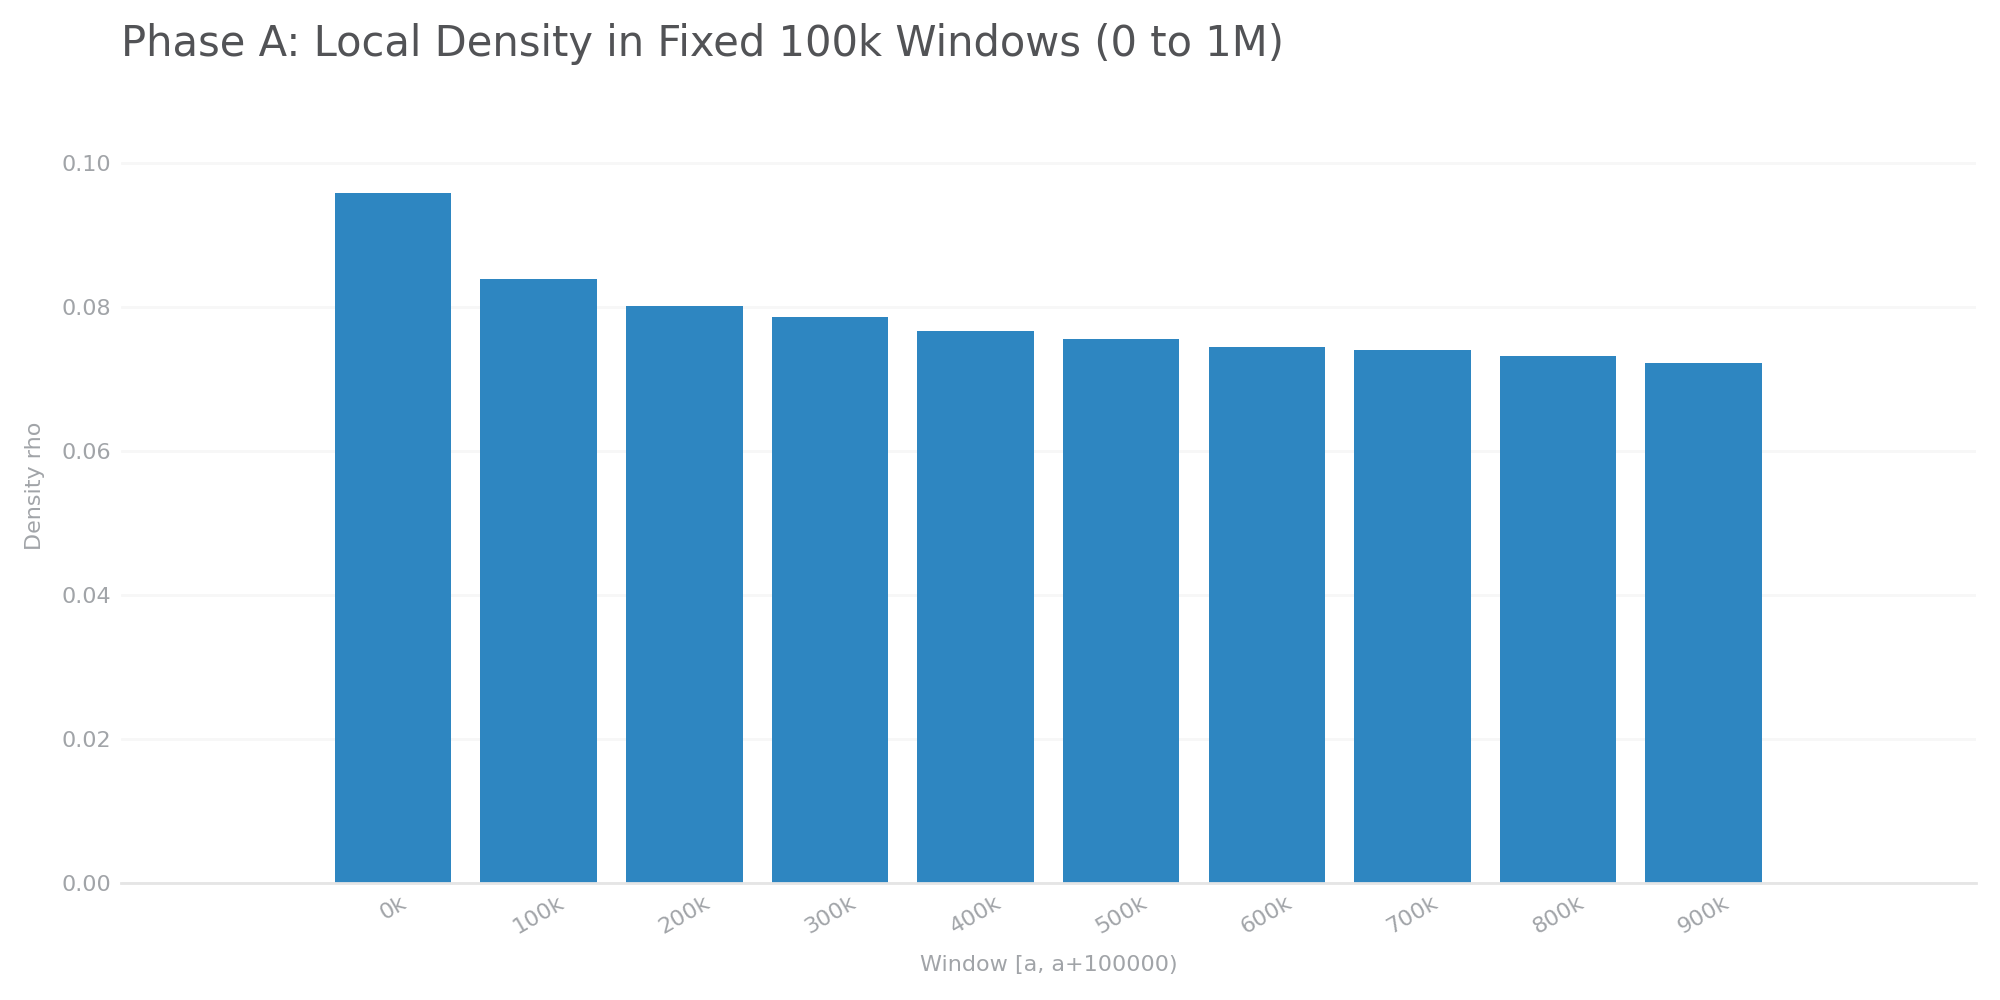
\includegraphics[width=0.90\textwidth]{prime1.png}
\caption{Official Research Identity Card — Prime}
\end{figure}

\begin{table}[H]
\centering
\begin{tabular}{ll}
\toprule
\textbf{Attribute} & \textbf{Verified Value} \\
\midrule
Author & Abdulla Mohammed Nasser Al-Jabri \\
Affiliation / Location & Sana'a, Republic of Yemen \\
ORCID & 0009-0003-3319-3822 \\
Email & \texttt{jabri62018@gmail.com} \\
Research Portal & \url{https://jabri-com.vercel.app} \\
Work Title & Edges of Counting and Computation — Prime \\
Mathematical Definition & $g_n = p_{n+1} - p_n$ \\
Computational Horizon & $N = 10^9$ ($\pi(10^9) = 50,847,534$) \\
Zenodo DOI & to be assigned on deposit \\
Date & November 21, 2026 \\
\bottomrule
\end{tabular}
\caption{Research Metadata and Reference Parameters}
\end{table}

% ==========================================
\section{Definitions and Mathematical Protocol}

\subsection{The Edge (Prime Gap)}
An edge $g_n$ is defined as the arithmetic difference between two consecutive primes:
\[
g_n = p_{n+1} - p_n, \quad \forall n \geq 1
\]
\begin{enumerate}
    \item \textbf{Sieve Protocol:} Primes are generated via the Sieve of Eratosthenes up to $N$, with $1$ explicitly excluded from the prime set.
    \item \textbf{Unique Odd Edge:} The initial edge $g_1 = 3 - 2 = 1$ is the sole odd gap in the sequence. Every prime $p_n > 2$ is odd, making every subsequent gap strictly even ($g_n \equiv 0 \pmod 2$ for all $n \geq 2$).
\end{enumerate}

\subsection{Counting, Deviation, and Density Functions}
\begin{itemize}
    \item $\pi(x)$: Exact count of primes $\leq x$.
    \item $\mathrm{Li}(x) = \mathrm{Ei}(\ln x) - \mathrm{Ei}(\ln 2) = \int_2^x \frac{dt}{\ln t}$: Offset logarithmic integral.
    \item $D_1(x) = \pi(x) - \mathrm{Li}(x)$ and $D_2(x) = \pi(x) - x/\ln x$.
    \item $R(x) = |D_1(x)| / \pi(x)$: Relative logarithmic deviation.
    \item $\rho_k = (\pi(b_k) - \pi(a_k)) / 10^8$ and $\bar{g}_k = 1/\rho_k$: Local density and mean gap in window $k$.
\end{itemize}

\subsection{Stage $D$ Inclusion Rule and $M1$ Size Classes}
A gap $g_n = p_{n+1} - p_n$ is counted inside Stage $D$ if and only if its upper endpoint satisfies $p_{n+1} > 10^8$ ($100\text{M}$), yielding exactly $45,086,079$ gaps in Stage $D$. Gaps are partitioned into three exhaustive $M1$ classes:
\begin{itemize}
    \item \textbf{Small:} $g \leq 6$ ($\{1, 2, 4, 6\}$).
    \item \textbf{Medium:} $8 \leq g \leq 14$ ($\{8, 10, 12, 14\}$).
    \item \textbf{Large:} $g \geq 16$.
\end{itemize}
Because $g_1 = 1$ falls inside the Small class and all subsequent gaps are even, no odd integers ($7$ or $15$) exist between class boundaries.

% ==========================================
\section{Cross-Stage Synthesis ($A \rightarrow D$) and Results}

\subsection{Closure Comparison Across Stages $A$--$D$}
\begin{table}[H]
\centering
\small
\begin{tabular}{llrrrrr}
\toprule
\textbf{Stage} & \textbf{Range} & \textbf{Window} & $\pi(x)$ & $D_1 = \pi - \mathrm{Li}$ & $D_2 = \pi - x/\ln x$ & $R = |D_1|/\pi$ \\
\midrule
$A$ & Up to $10^6$ & $10^5$ & $78,498$ & $-128.504$ & $+6,115.586$ & $0.001637035$ \\
$B$ & Up to $10^7$ & $10^6$ & $664,579$ & $-338.360$ & $+44,158.312$ & $0.000509134$ \\
$C$ & Up to $10^8$ & $10^7$ & $5,761,455$ & $-753.330$ & $+332,773.976$ & $0.000130753$ \\
$D$ & $10^8 \rightarrow 10^9$ & $10^8$ & $50,847,534$ & $-1,699.912$ & $+2,592,591.566$ & $0.000033432$ \\
\bottomrule
\end{tabular}
\caption{Closure comparison across Stages $A, B, C,$ and $D$}
\end{table}

\subsection{Stage $D$ Cumulative Checkpoints (Every $100\text{M}$)}
\begin{table}[H]
\centering
\small
\begin{tabular}{rrrrrrr}
\toprule
$x$ & $\pi(x)$ & $\mathrm{Li}(x)$ & $D_1$ & $\Delta D_1$ & $D_2$ & $R(x)$ \\
\midrule
$100{,}000{,}000$ & $5{,}761{,}455$ & $5{,}762{,}208.3$ & $-753.3$ & $-753.3$ & $332{,}774.0$ & $0.000131$ \\
$200{,}000{,}000$ & $11{,}078{,}937$ & $11{,}079{,}973.8$ & $-1{,}036.8$ & $-283.5$ & $615{,}308.2$ & $0.000094$ \\
$300{,}000{,}000$ & $16{,}252{,}325$ & $16{,}253{,}408.1$ & $-1{,}083.1$ & $-46.3$ & $882{,}915.9$ & $0.000067$ \\
$400{,}000{,}000$ & $21{,}336{,}326$ & $21{,}337{,}377.0$ & $-1{,}051.0$ & $+32.1$ & $1{,}141{,}420.0$ & $0.000049$ \\
$500{,}000{,}000$ & $26{,}355{,}867$ & $26{,}356{,}831.1$ & $-964.1$ & $+86.9$ & $1{,}393{,}458.7$ & $0.000037$ \\
$600{,}000{,}000$ & $31{,}324{,}703$ & $31{,}326{,}044.207$ & $-1{,}341.207$ & $-377.103$ & $1{,}640{,}014.082$ & $0.000042816$ \\
$700{,}000{,}000$ & $36{,}252{,}931$ & $36{,}254{,}240.999$ & $-1{,}309.999$ & $+31.208$ & $1{,}882{,}917.694$ & $0.000036135$ \\
$800{,}000{,}000$ & $41{,}146{,}179$ & $41{,}147{,}861.2$ & $-1{,}682.2$ & $-372.2$ & $2{,}122{,}021.5$ & $0.000041$ \\
$900{,}000{,}000$ & $46{,}009{,}215$ & $46{,}011{,}647.6$ & $-2{,}432.6$ & $-750.4$ & $2{,}357{,}836.0$ & $0.000053$ \\
$1{,}000{,}000{,}000$ & $50{,}847{,}534$ & $50{,}849{,}233.912$ & $-1{,}699.912$ & $+732.688$ & $2{,}592{,}591.566$ & $0.000033432$ \\
\bottomrule
\end{tabular}
\caption{Cumulative checkpoints across Stage $D$}
\end{table}

\subsection{Window Density and Top 15 Gap Frequencies in Stage $D$}
Across the nine $100\text{M}$ windows of Stage $D$, local prime density $\rho_k$ declined steadily from $0.053175$ ($100\text{M}$--$200\text{M}$) to $0.048383$ ($900\text{M}$--$1\text{B}$), while the mean gap $\bar{g}_k$ rose from $18.806$ to $20.668$. The maximum observed gap inside Stage $D$ was $g = 282$ between $436{,}273{,}009$ and $436{,}273{,}291$.

\begin{table}[H]
\centering
\begin{tabular}{rrr}
\toprule
\textbf{Rank} & \textbf{Gap} & \textbf{Count in $D$} \\
\midrule
1 & 6 & $5{,}321{,}039$ \\
2 & 12 & $3{,}930{,}575$ \\
3 & 10 & $3{,}054{,}751$ \\
4 & 4 & $2{,}984{,}422$ \\
5 & 2 & $2{,}984{,}194$ \\
6 & 18 & $2{,}966{,}294$ \\
7 & 8 & $2{,}360{,}929$ \\
8 & 14 & $2{,}171{,}364$ \\
9 & 24 & $2{,}109{,}926$ \\
10 & 30 & $1{,}955{,}144$ \\
11 & 16 & $1{,}630{,}293$ \\
12 & 20 & $1{,}621{,}121$ \\
13 & 22 & $1{,}393{,}734$ \\
14 & 28 & $1{,}089{,}676$ \\
15 & 36 & $1{,}057{,}496$ \\
\bottomrule
\end{tabular}
\caption{Top 15 prime gap frequencies in Stage $D$ — Total in $D$: $45,086,079$}
\end{table}

\subsection{Visual Diagnostics ($B$, $C$, and $D$)}
\begin{figure}[H]
\centering
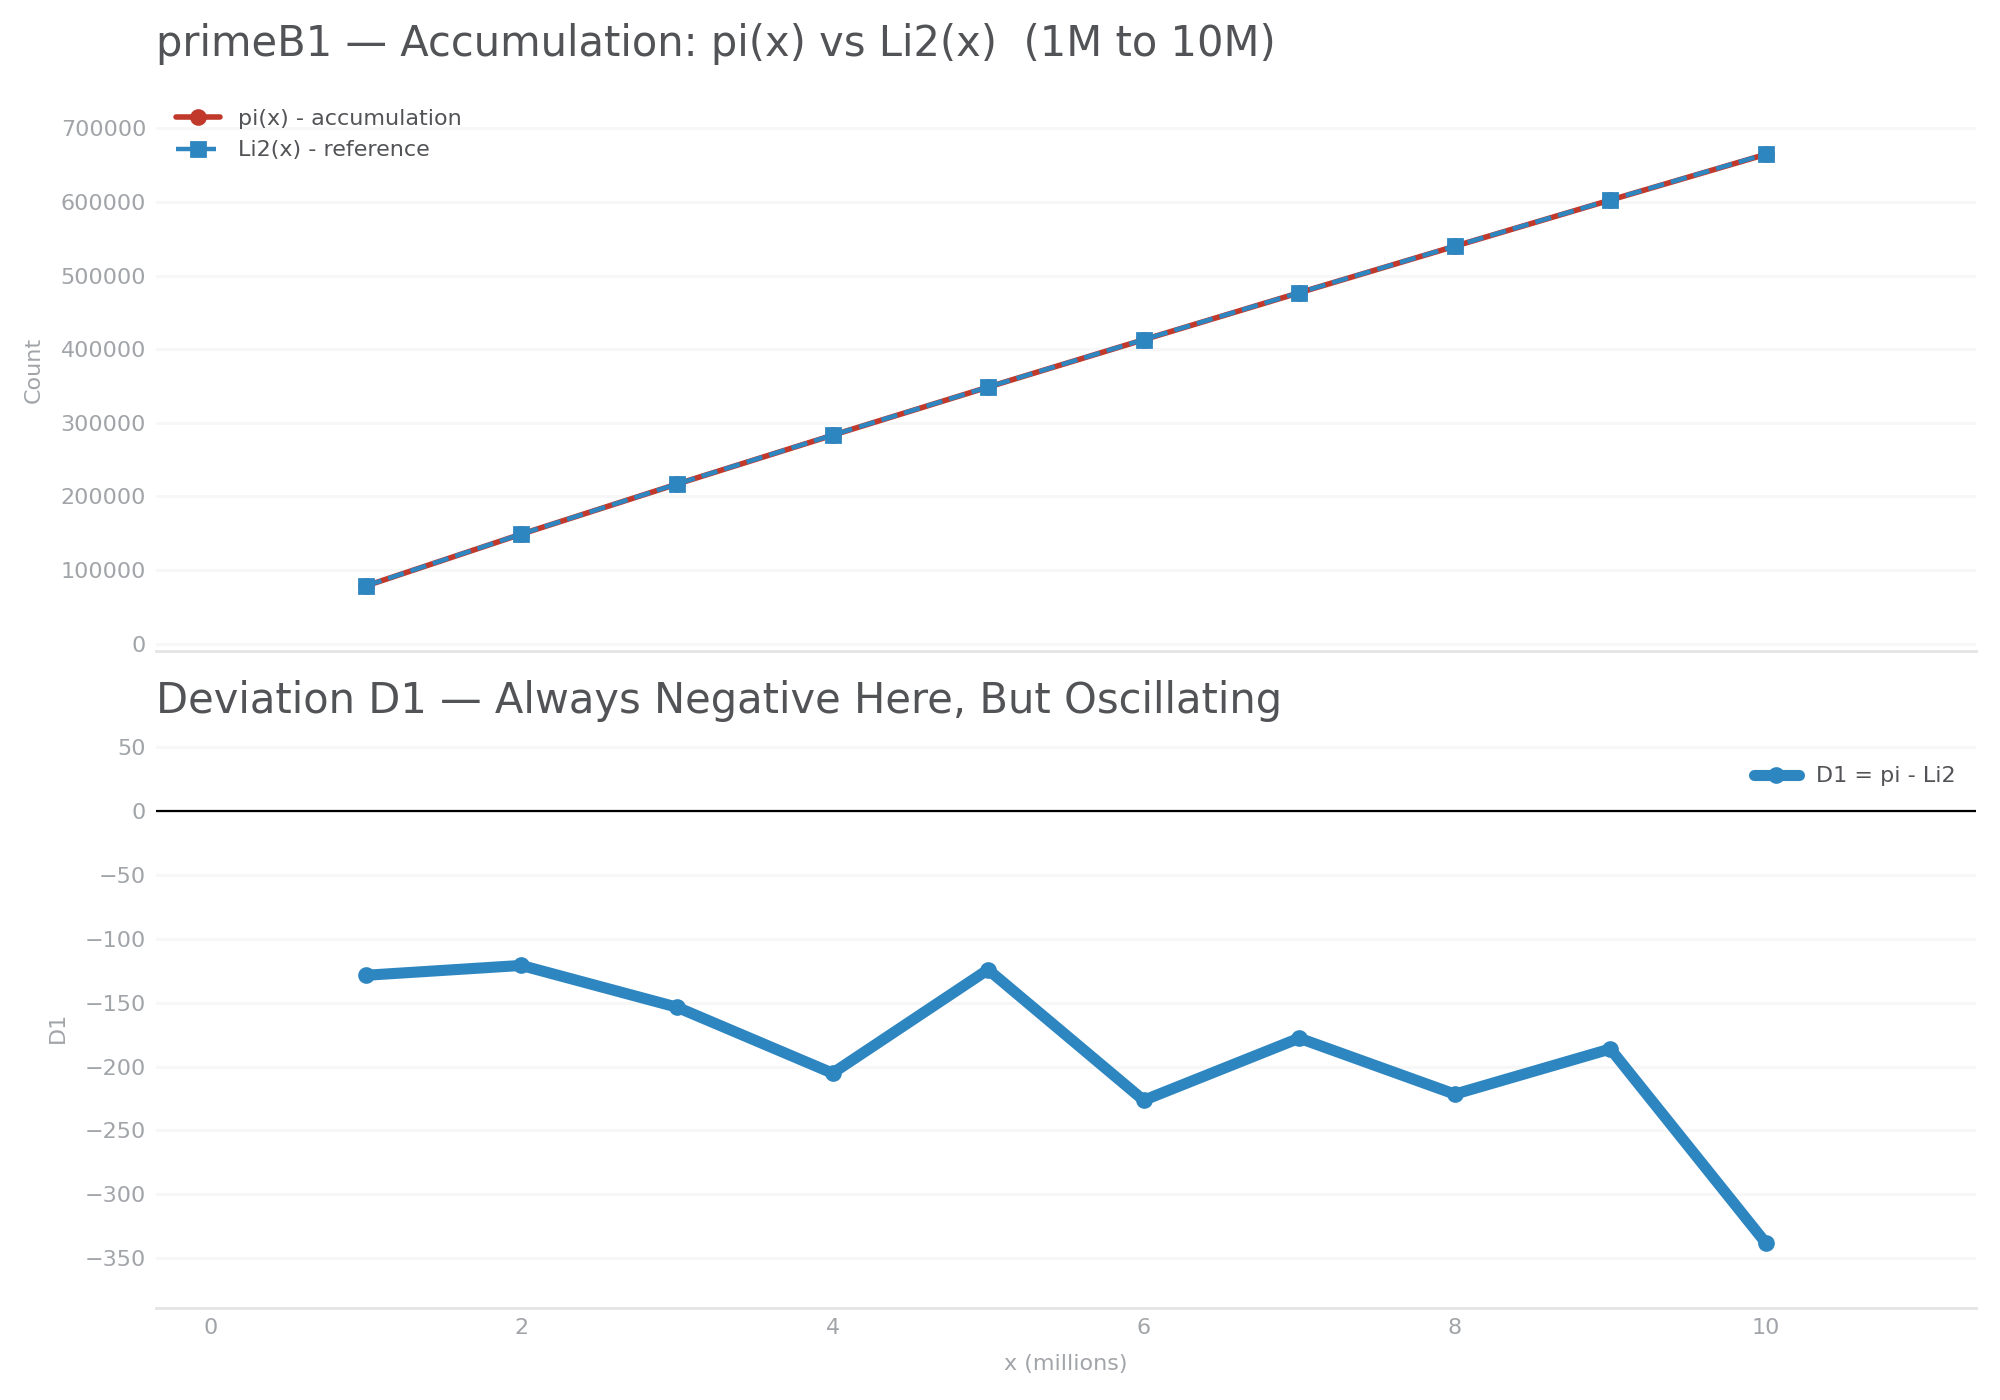
\includegraphics[width=0.32\textwidth]{primeB1.png}
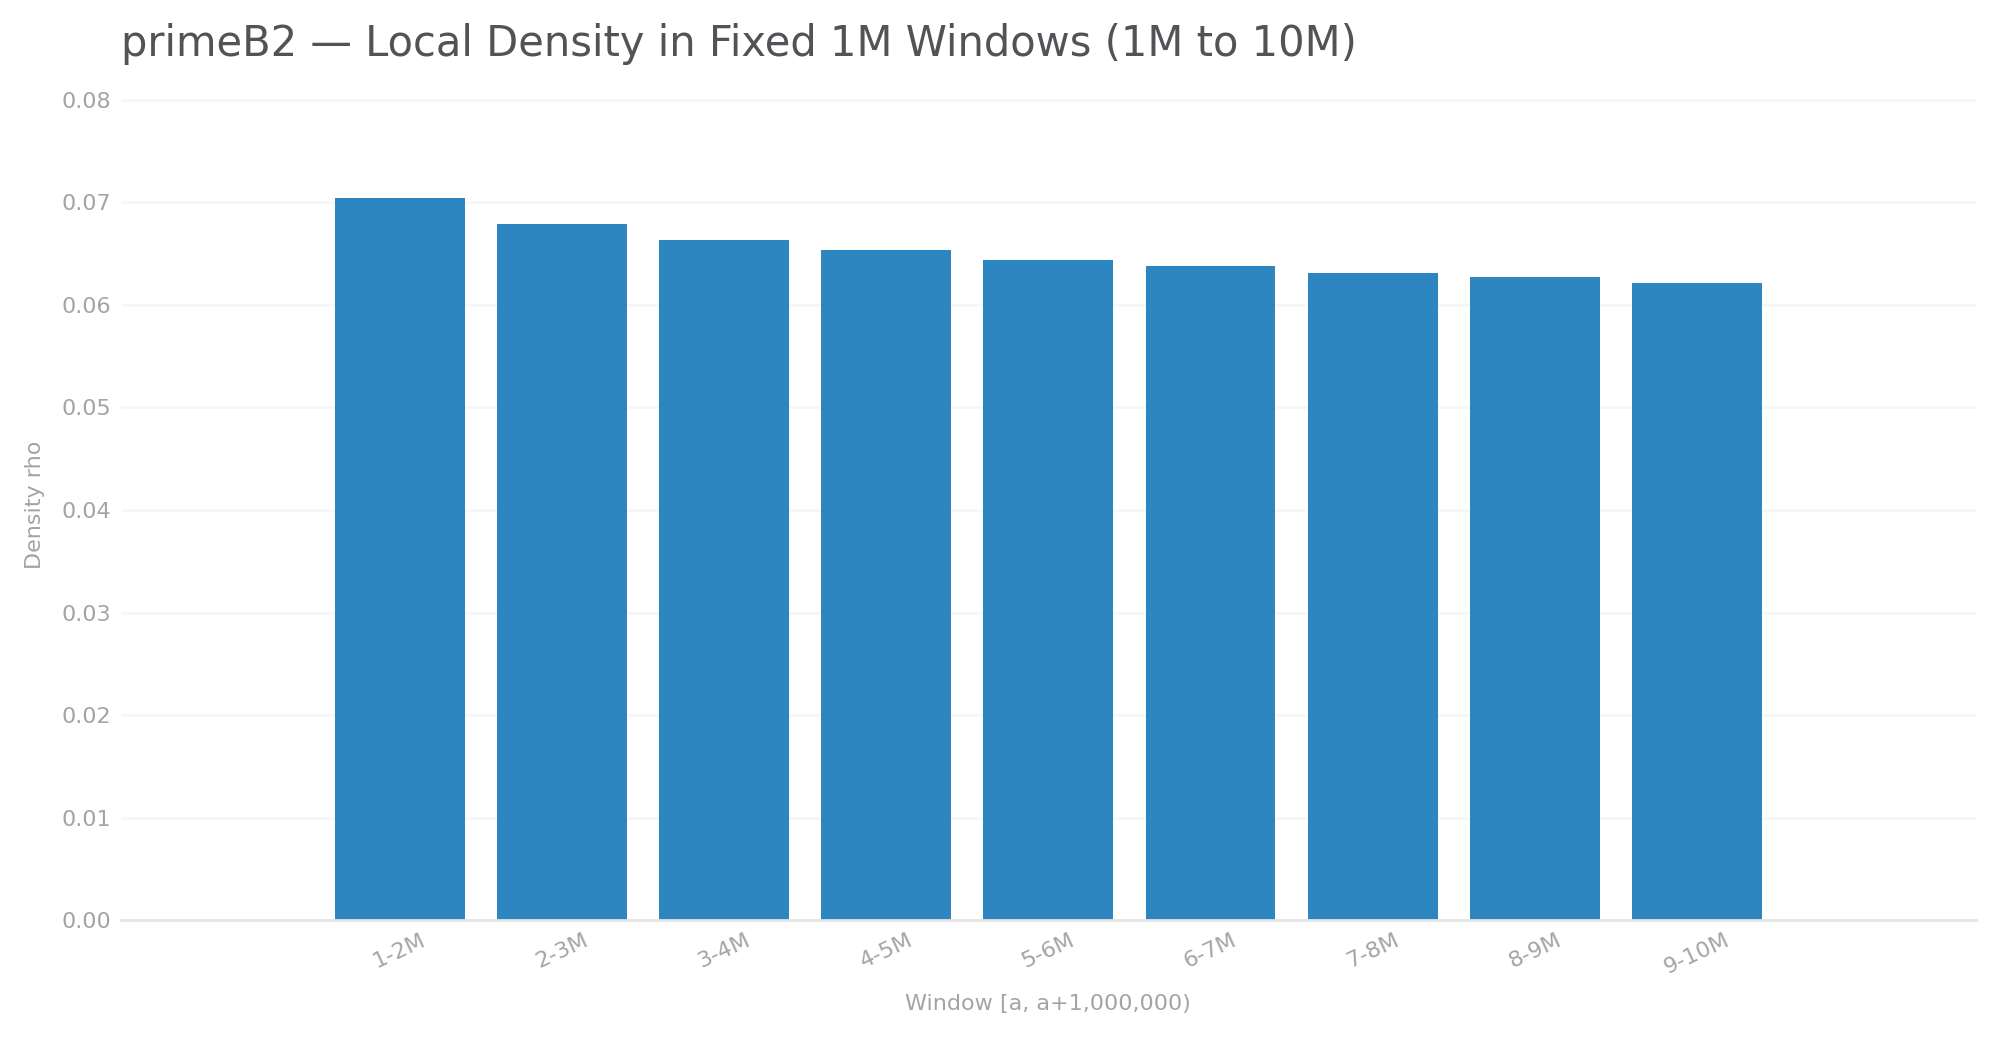
\includegraphics[width=0.32\textwidth]{primeB2.png}
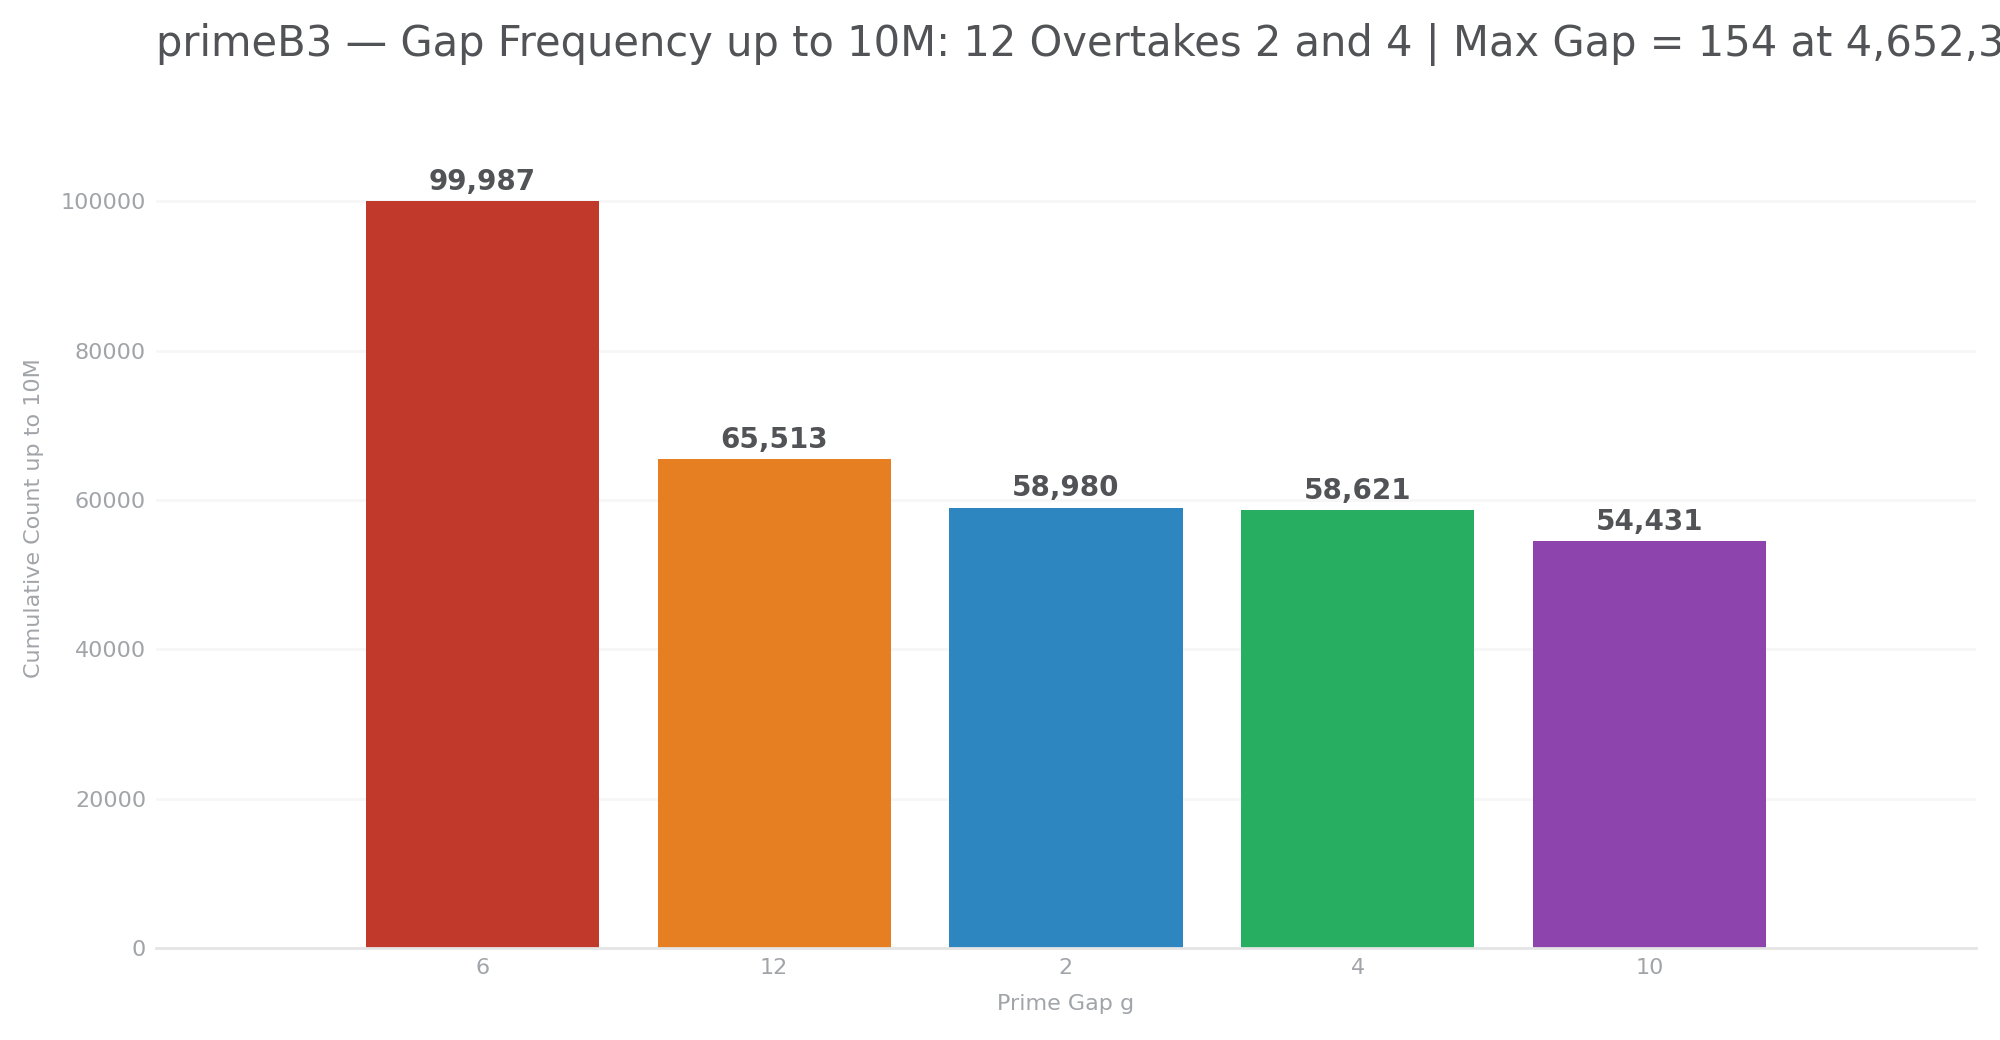
\includegraphics[width=0.32\textwidth]{primeB3.png}
\caption{Stage $B$: Deviation $D_1$, Density $\rho_k$, and Gap Frequencies}
\end{figure}
\begin{figure}[H]
\centering
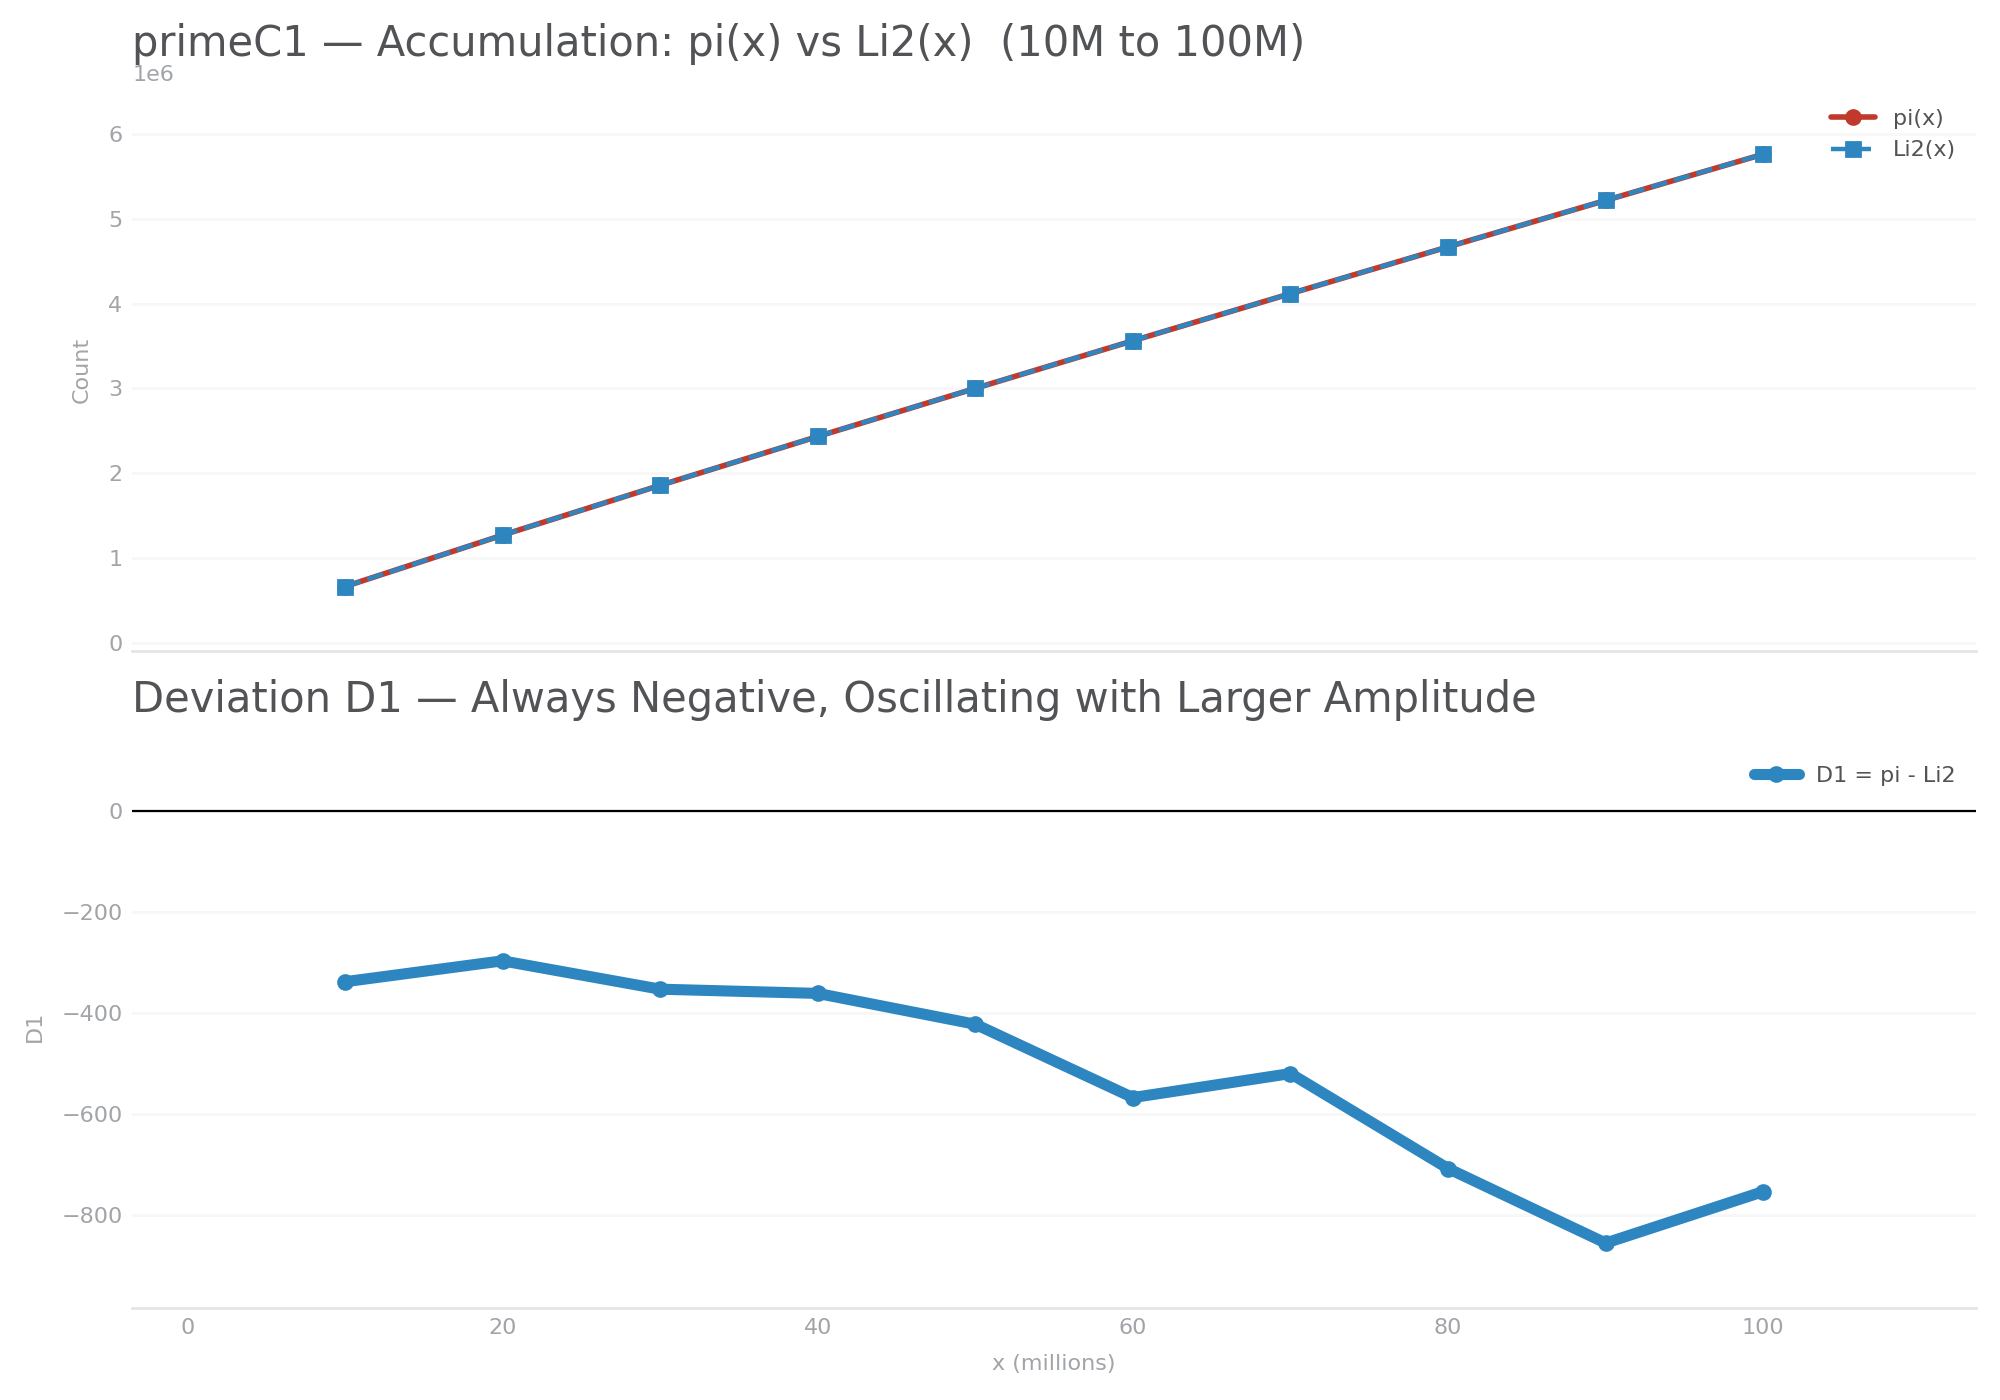
\includegraphics[width=0.32\textwidth]{primeC1.png}
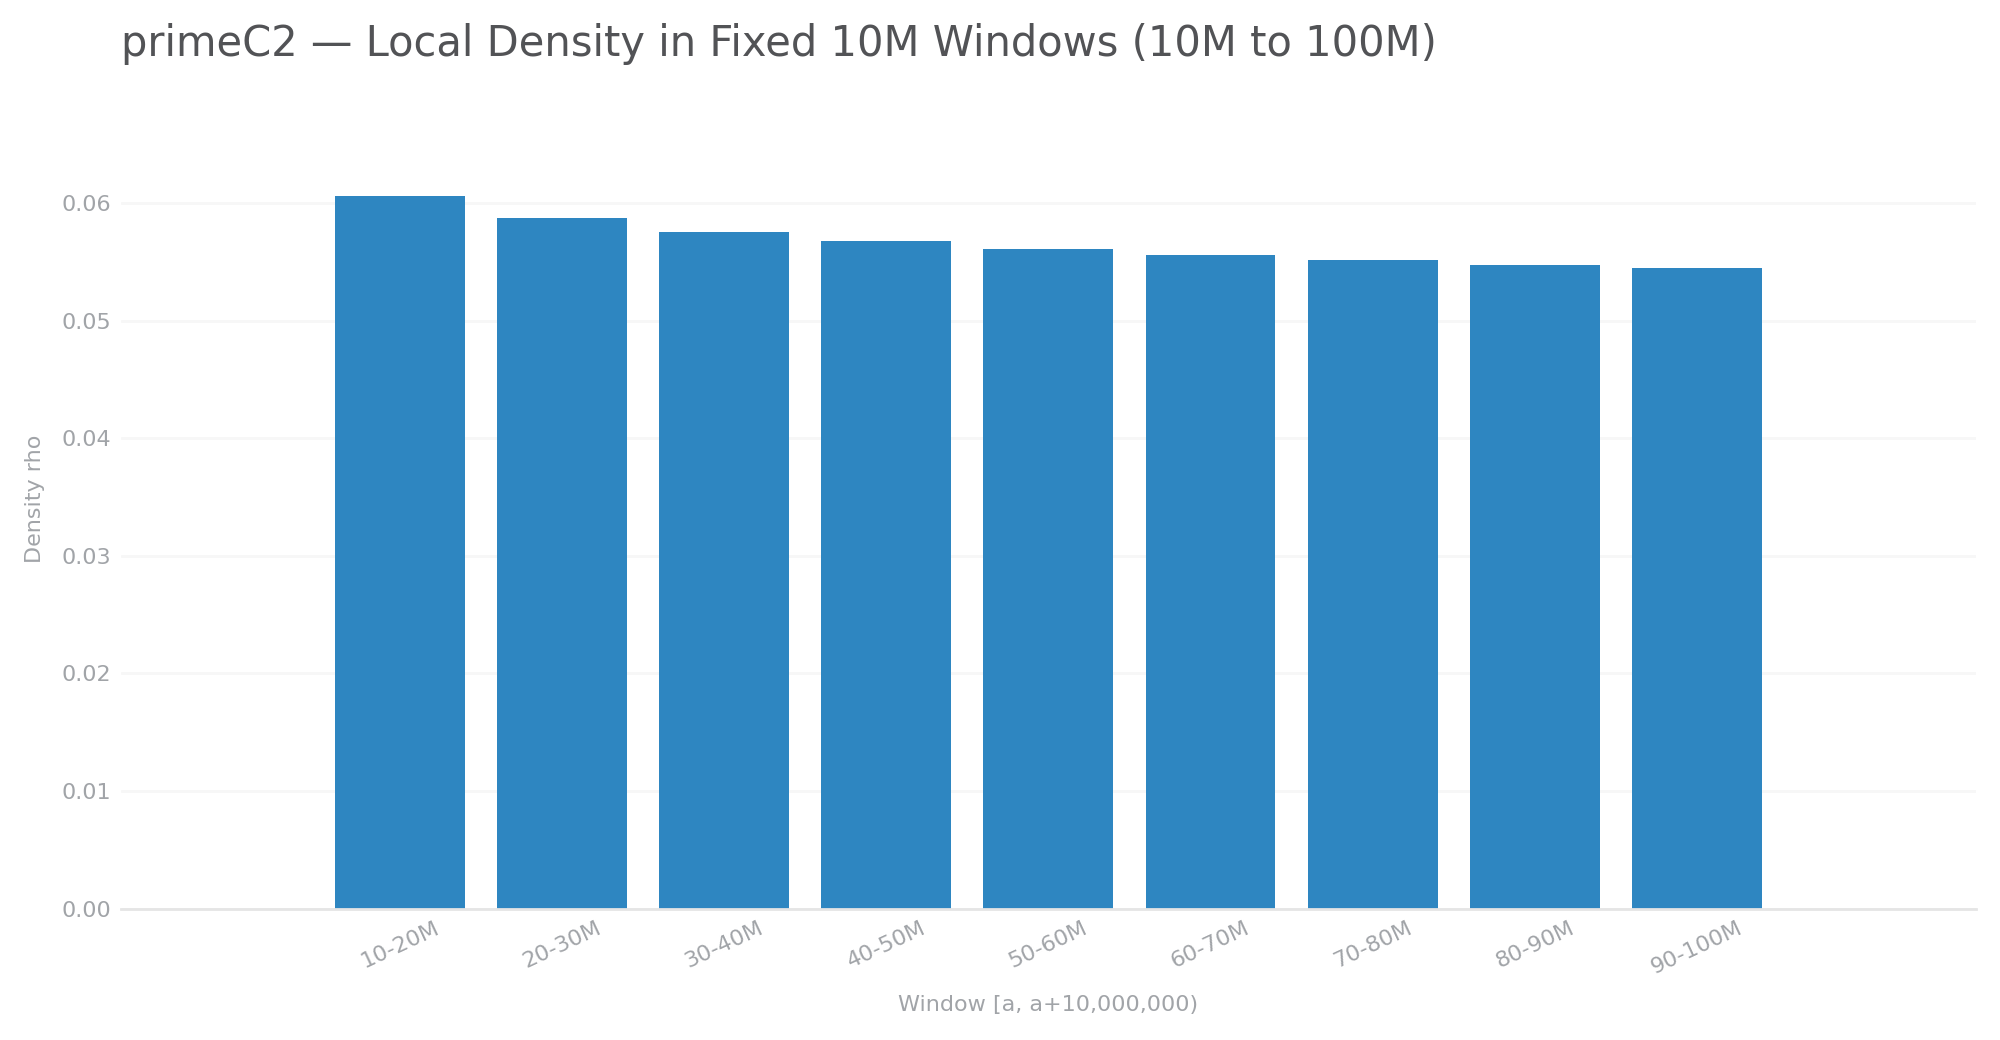
\includegraphics[width=0.32\textwidth]{primeC2.png}
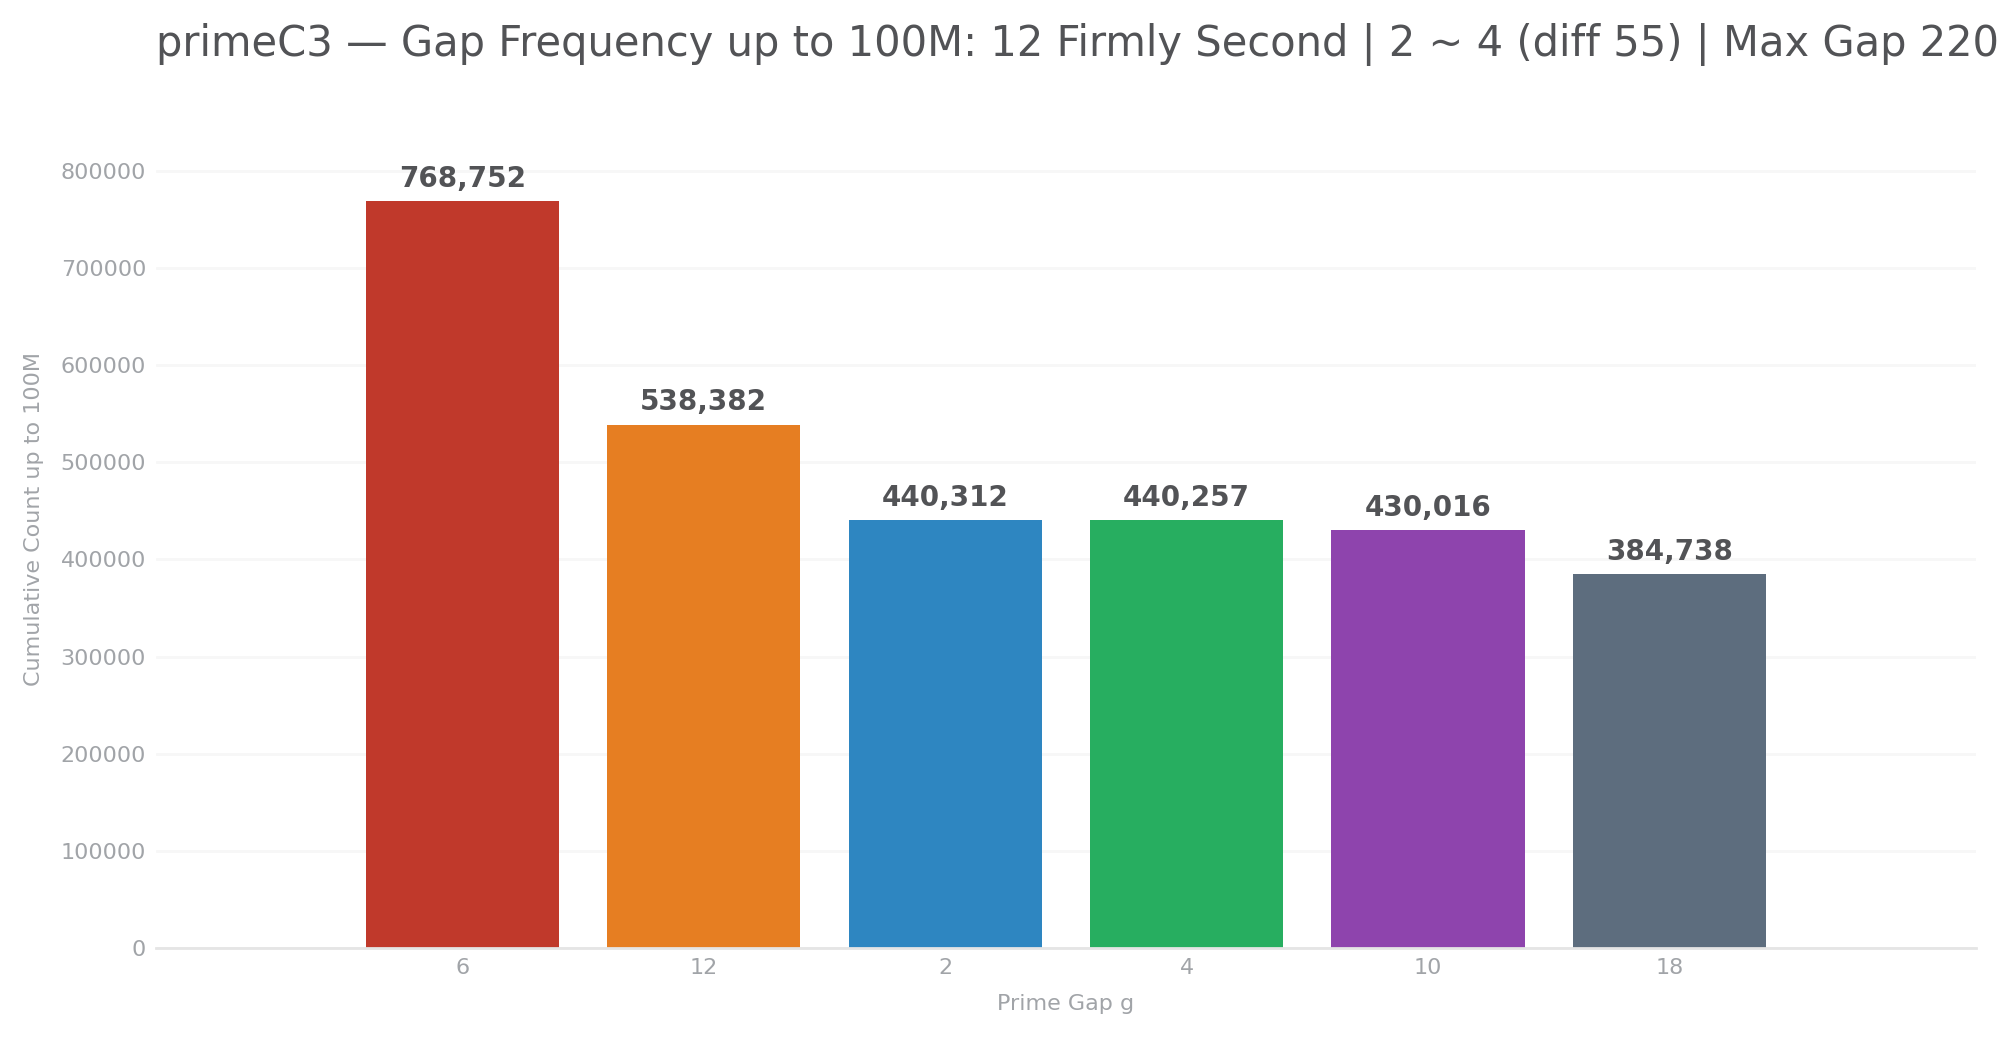
\includegraphics[width=0.32\textwidth]{primeC3.png}
\caption{Stage $C$: Deviation $D_1$, Density $\rho_k$, and Gap Frequencies}
\end{figure}
\begin{figure}[H]
\centering
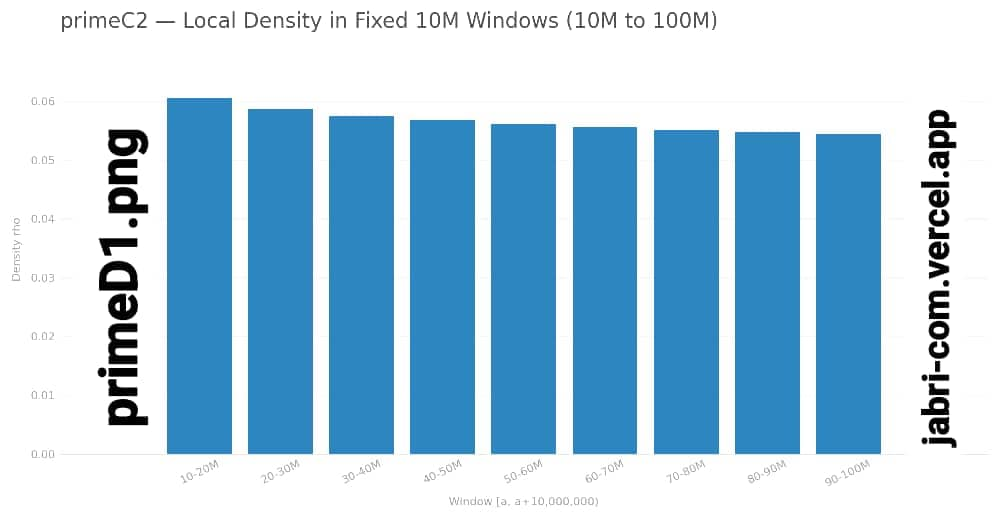
\includegraphics[width=0.32\textwidth]{primeD1.png}
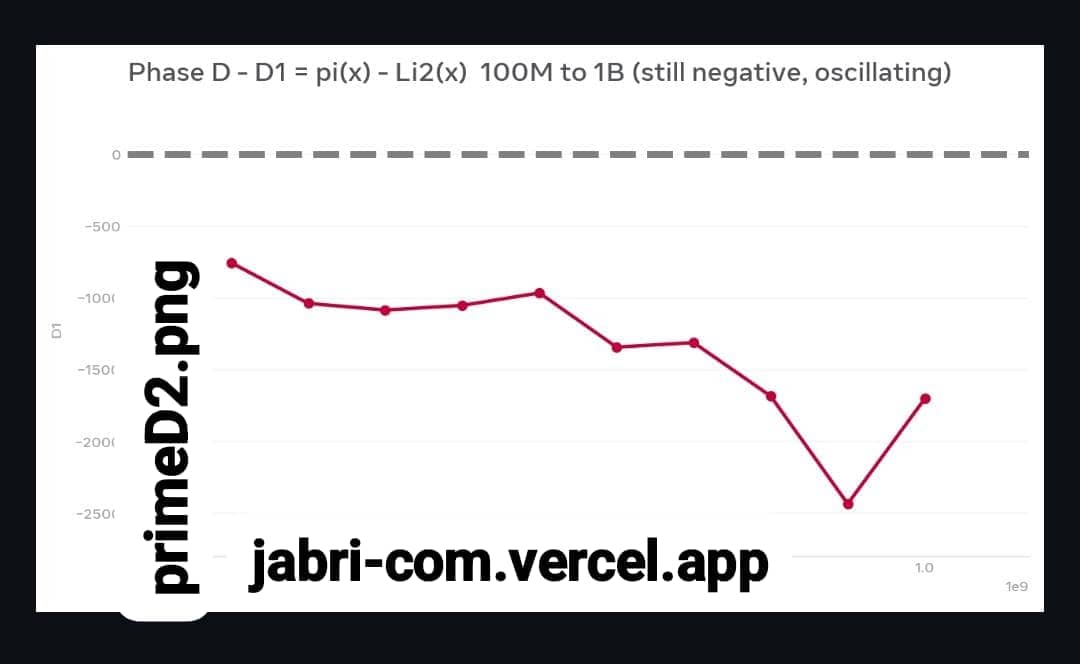
\includegraphics[width=0.32\textwidth]{primeD2.png}
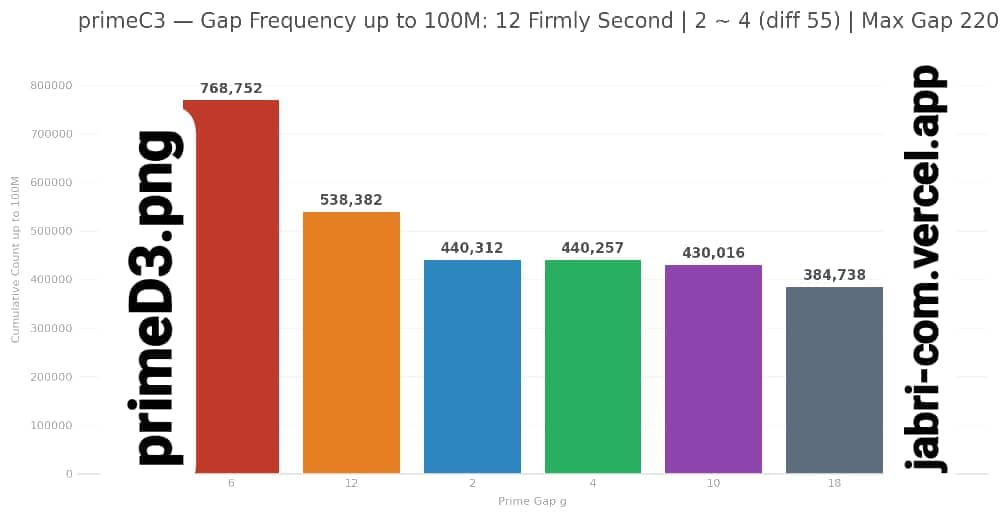
\includegraphics[width=0.32\textwidth]{primeD3.png}
\caption{Stage $D$: Deviation $D_1$, Density $\rho_k$, and Gap Frequency Shift}
\end{figure}

% ==========================================
\section{Cross-Stage Synthesis: Adjacency Structure and Primorial Sieve}
\subsection{Central Question}
Can the negative lag-1 autocorrelation of adjacent prime gaps ($\rho_1 < 0$) be derived directly from small-prime divisibility constraints, without assuming gap independence or a prior asymptotic law? This section is limited to the first $1,000,000$ primes ($p_{10^6} = 15,485,863$). No $N = 10,000,000$ computation is claimed, and no Hurst / DFA estimate is reported as proven.

\subsection{Adjacency Measures}
\[
\rho_k = \frac{\sum_{i=1}^{n-k} (g_i - \bar{g})(g_{i+k} - \bar{g})}{\sum_{i=1}^{n} (g_i - \bar{g})^2}
\qquad
R_{\text{stat}} = \frac{1}{n-1} \sum_{i=1}^{n-1} \frac{\min(g_i, g_{i+1})}{\max(g_i, g_{i+1})}
\]
A shuffled control (random reordering of the gap vector) drives $\rho_1$ to approximately $0$, showing the negative value depends on the original adjacency order.

\subsection{Primorial Sieve Model}
For $M = \prod_{p \le p_k} p$, e.g. $M = 6, 30, 210, 2310, 30030, 510510$, the exact cycle of residues coprime to $M$ gives a closed gap cycle. For $M = 30$ ($\phi(30) = 8$):
\[
\mathcal{C}_{30} = [6, 4, 2, 4, 2, 4, 6, 2]
\]
These purely arithmetic cycles already have $r_{\text{sieve}} < 0$. Part of the repulsion between adjacent gaps is therefore a forced modular effect, not a purely random phenomenon. This does not prove a general asymptotic law.

% ==========================================
\section{Discussion, Methodological Verification, and Limitations}
\subsection{What Changed vs. What Remained Invariant}
\begin{itemize}
\item \textbf{Invariants:} $D_1 < 0$ and $D_2 > 0$ held at every closure point from $A$ to $D$; gaps $6$ and $12$ retained Ranks $1$ and $2$ across all stages.
\item \textbf{Rank Shift in Stage $D$:} Up to Stage $C$, the cumulative top six gaps were ordered $(6, 12, 2, 4, 10, 18)$. Inside Stage $D$ alone, the ranking shifted to $(6, 12, 10, 4, 2, 18)$, with gap $10$ advancing to Rank $3$ and gaps $4$ and $2$ converging to within a difference of just $228$ occurrences ($2{,}984{,}422$ vs. $2{,}984{,}194$).
\item \textbf{Primorial Modular Constraint:} Modular sieving by small primorials imposes an inherent negative lag-1 autocorrelation ($r_{\text{sieve}} < 0$), explaining why consecutive gaps repel each other locally ($r = -0.03006$ in $M1$) without enabling deterministic prediction.
\end{itemize}
\subsection{Isolation of Verification Sieve Artifacts}
During independent verification of Stage $D$, a defective verification script that erroneously included $1$ as a prime nearly introduced an unwarranted adjustment. Isolating and discarding that artifact — strictly enforcing $1 \notin \mathbb{P}$ — was integral to validating the exact Stage $D$ gap count ($45{,}086{,}079$).
\subsection{Explicit Scope Boundaries (What Was Not Proven)}
Stages $A$--$D$ do \textbf{not} prove that $D_1(x)$ remains negative beyond $10^9$, nor do they establish any periodic law from $\Delta D_1$ fluctuations ($-750.4$ to $+732.688$), nor do they prove whether the near-tie between gaps $2$ and $4$ persists or reverses in Stage $E$ ($1\text{B} \rightarrow 10\text{B}$).

% ==========================================
\section{Committee Questions}
\textbf{Why exclude 1?} Because $1$ is not prime; including it creates a false gap.

\textbf{Why is gap 1 the only odd gap?} After $2$, all primes are odd, and the difference of two odds is even.

\textbf{Can you predict the next gap?} No, $r = -0.03006$ is too weak for prediction.

\textbf{Did you claim a general law?} No, observation up to $10^9$ only, no theorem, no conjecture.

% ==========================================
\section{Reproducibility and Conclusion}
All computations were executed in \texttt{Python 3} using an exact Sieve of Eratosthenes ($1$ excluded, $M1$-$E$ seed: \texttt{SEED = 20261120}). While consecutive prime gaps up to $10^9$ carry no deterministic predictive memory ($r = -0.03006$), their frequency hierarchy undergoes measurable structural reorganization driven by decreasing local density.

\begin{thebibliography}{9}
\bibitem{hardy} G. H. Hardy and E. M. Wright, \textit{An Introduction to the Theory of Numbers}, 6th ed., Oxford University Press, 2008.
\bibitem{lemke} R. J. Lemke Oliver and K. Soundararajan, ``Unexpected biases in the distribution of consecutive primes,'' \textit{PNAS}, vol. 113, no. 31, pp. E4446--E4454, 2016.
\bibitem{granville} A. Granville, ``Harald Cram\'er and the distribution of prime numbers,'' \textit{Scandinavian Actuarial Journal}, vol. 1995, no. 1, pp. 12--28, 1995.
\end{thebibliography}
\end{document}
